\documentclass[12pt, twoside]{article}
\usepackage[letterpaper, margin=1in, headsep=0.5in]{geometry}
\usepackage[english]{babel}
\usepackage[utf8]{inputenc}
\usepackage{amsmath}
\usepackage{amsfonts}
\usepackage{amssymb}
\usepackage{tikz}
\usetikzlibrary{quotes, angles}
\usepackage{graphicx}
%\usepackage{pgfplots}
%\pgfplotsset{width=10cm,compat=1.9}
%\usepgfplotslibrary{statistics}
%\usepackage{pgfplotstable}
%\usepackage{tkz-fct}
%\usepackage{venndiagram}
\usepackage{multicol}


\usepackage{fancyhdr}
\pagestyle{fancy}
\fancyhf{}
\fancyhead[RE]{\thepage}
\fancyhead[RO]{\thepage \\Name: \hspace{4cm} \, \\}
\fancyhead[LO]{BECA / Dr. Huson / Geometry 10th Grade\\* Unit 6: Analytic Geometry \\ 27 November 2019}

\renewcommand{\headrulewidth}{0pt}

\begin{document}
\subsubsection*{6.3 Classwork: Due at end of class}
  \begin{enumerate}

\subsubsection*{Do Not Solve! \\
Model the situation with an equation in terms of $x$.}

  \item Given $\overline{ABC}$, with $AB=2x-1$, $BC=3x+3$, and $AC=17$. Find $x$. \vspace{1cm}
  \begin{flushright}
    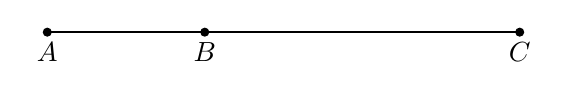
\begin{tikzpicture}
      \draw [-, thick] (0,0) node[below]{$A$}--
      (2,0) node[below]{$B$}--
      (6,0) node[below]{$C$};
      \draw [fill] (0,0) circle [radius=0.05];
      \draw [fill] (2,0) circle [radius=0.05];
      \draw [fill] (6,0) circle [radius=0.05];
    \end{tikzpicture}
    \end{flushright} \vspace{1cm}

  \item Given $m\angle 3 = x+30$ and $m\angle 5 = 4x-20$. Find $x$. 
  \begin{flushright}
  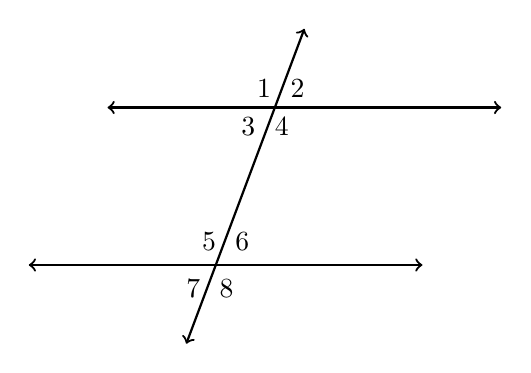
\begin{tikzpicture}
    \draw [<->, thick] (3,2)--(8,2);
    \draw [<->, thick] (2,0)--(7,0);
    \draw [<->, thick] (4,-1)--(5.5,3);
    \node at (4.5,0.3) [left]{$5$};
    \node at (4.5,0.3) [right]{$6$};
    \node at (4.3,-0.3) [left]{$7$};
    \node at (4.3,-0.3) [right]{$8$};
    \node at (5.2,2) [above left]{$1$};
    \node at (5.2,2) [above right]{$2$};
    \node at (5,2) [below left]{$3$};
    \node at (5,2) [below right]{$4$};
  \end{tikzpicture}
  \end{flushright} \vspace{0.5cm}

  \item In the diagram below $m\angle AOB = 6x+5$ and $m\angle COB = 8x+15$. Find $x$. %\vspace{0.25cm}
  \begin{flushright}
  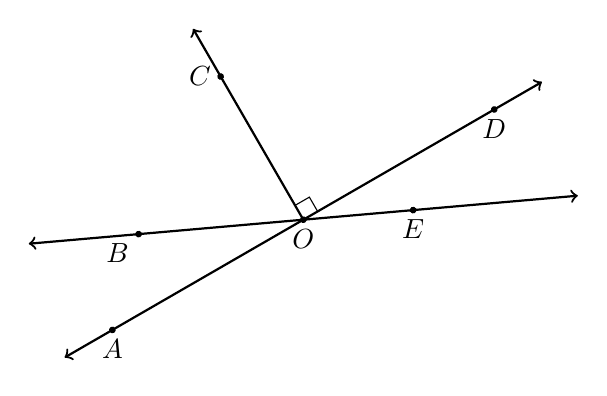
\begin{tikzpicture}[scale=0.7, rotate=30]
  \draw [<->, thick] (-25:5)--(0,0)--(155:5);
  \draw [<->, thick] (-5,0)--(5,0);
  \draw [->, thick] (0,0)--(0,4);
  \draw (0,0)++(0.3,0)--++(0,0.3)--+(-0.3,0);
  %\draw [fill] (-1,2.5) circle [radius=0.05] node[left ]{$B$};
  \draw [fill] (155:3) circle [radius=0.05] node[below left]{$B$};
  \draw [fill] (-4,0) circle [radius=0.05] node[below]{$A$}; 
  \draw [fill] (0,0) circle [radius=0.05] node[below]{$O$};
  \draw [fill] (0,3) circle [radius=0.05] node[left]{$C$};
  \draw [fill] (4,0) circle [radius=0.05] node[below]{$D$};
  \draw [fill] (-25:2) circle [radius=0.05] node[below]{$E$};
  \end{tikzpicture}
  \end{flushright}

  \item The point $K$ is the midpoint of $\overline{JL}$, $JK=3x+15$, and $JL=9x+9$. Find $x$.  \vspace{1cm}
  \begin{flushright}
    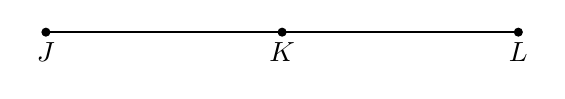
\begin{tikzpicture}
      \draw [-, thick] (0,0) node[below]{$J$}--
      (3,0) node[below]{$K$}--
      (6,0) node[below]{$L$};
      \draw [fill] (0,0) circle [radius=0.05];
      \draw [fill] (3,0) circle [radius=0.05];
      \draw [fill] (6,0) circle [radius=0.05];
    \end{tikzpicture}
    \end{flushright} \vspace{2cm}

\newpage
  \item On the graph below, $\overleftrightarrow{AB}$ is shown with A(0, 4), B(3,0). A dilation of $k=2$ centered at the origin maps $\overleftrightarrow{AB} \rightarrow \overleftrightarrow{A'B'}$.\\*[0.5cm]
  Draw $\overleftrightarrow{A'B'}$ on the graph, labeling $A'$ and $B'$.
    \begin{center}
      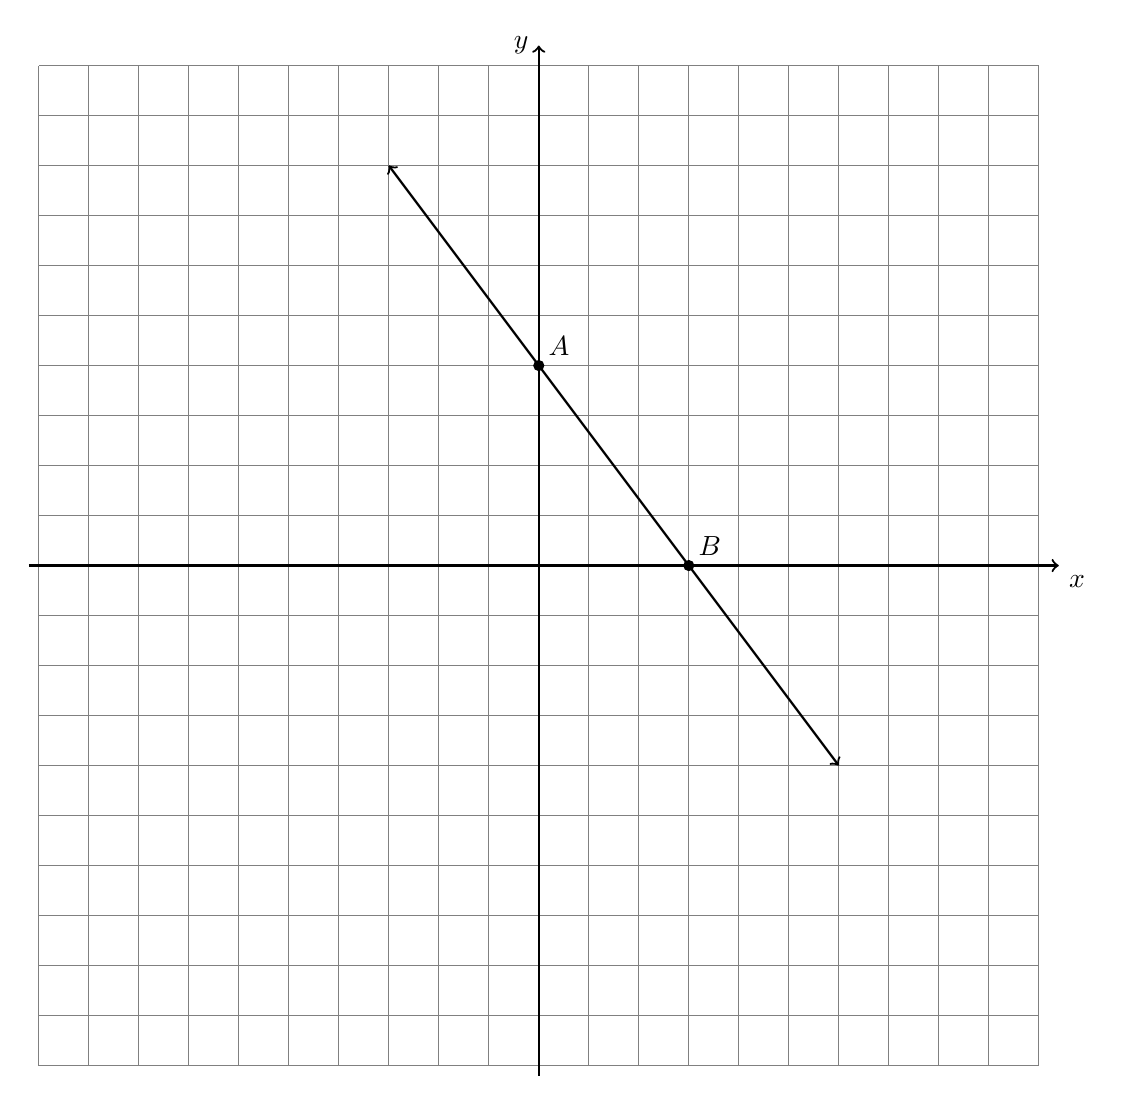
\begin{tikzpicture}[scale=.635]
        \draw [help lines] (-10,-10) grid (10,10);
        \draw [thick, ->] (-10.2,0) -- (10.4,0) node [below right] {$x$};
        \draw [thick, ->] (0,-10.2)--(0,10.4) node [left] {$y$};
        \draw [thick, <->] (-3,8)--(6,-4);
        \draw [fill] (0, 4) circle[radius = 0.1] node[above right]{$A$};
        \draw [fill] (3, 0) circle[radius = 0.1] node[above right]{$B$};
      \end{tikzpicture}
    \end{center}
      \vspace{1cm}
    \begin{enumerate}
      \item Write down the equation $\overleftrightarrow{AB}$ \vspace{2cm}
      \item Write down the equation $\overleftrightarrow{A'B'}$
    \end{enumerate}

\newpage
  \item Triangle $ABC$ is dilated with a scale factor of $k = 1.25$ centered at $A$, yielding $\triangle ADE$, as shown. Given $AB=8$, $BC=12$, and $AC=16$. \\[0.25cm] Find $AD$, $DE$, and $CE$.
  \begin{flushright}
      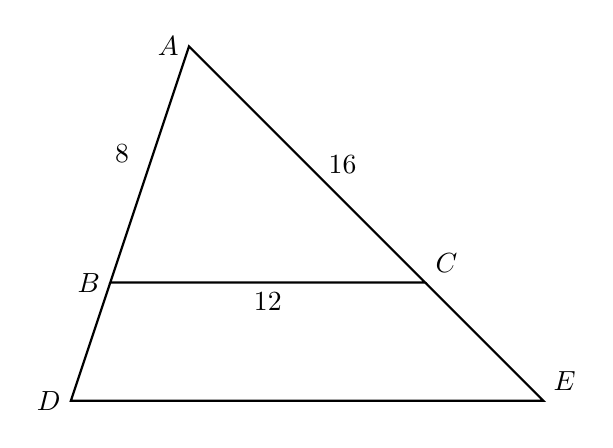
\begin{tikzpicture}[scale=0.5]
        \draw [thick]
        (0,0)node[left]{$B$}--
        (8,0)node[above right]{$C$}--
        (2,6)node[left]{$A$}--cycle;
        \draw [thick]
        (0,0)--
        (-1,-3)node[left]{$D$}--
        (11,-3)node[above right]{$E$}--(8,0);
        \node at (4,0)[below]{$12$};
        \node at (5.3, 3)[right]{$16$};
        \node at (0.3, 2.8)[above]{$8$};
      \end{tikzpicture}
    \end{flushright} \vspace{2.5cm}

  \item Find the image of $P(3,1)$ after the translation $(x,y) \rightarrow (x-1,y+12)$.  \vspace{2.5cm}

  \item A translation maps triangle $ABC$ onto triangle $PQR$. \vspace{0.5cm}
    \begin{multicols}{2}  
    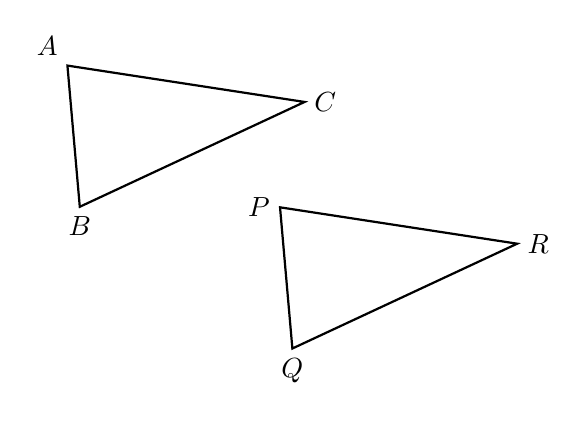
\begin{tikzpicture}[scale=0.9]
        \coordinate [label=above left:$A$](A) at (95:2);
        \coordinate [label=below:$B$](B) at (0, 0);
        \coordinate [label=right:$C$](C) at (25:3.5);
        \draw [thick] (A)--(B)--(C)--cycle;
  
        \draw [thick, xshift=3cm, yshift=-2cm] (95:2) node[left]{$P$}--
        (0,0) node[below]{$Q$}--
        (25:3.5) node[right]{$R$}--cycle;
      \end{tikzpicture}\\
      Write each corresponding object.
      \begin{enumerate}
        \item $B \rightarrow$ \rule{2cm}{0.15mm}
        \item $\angle C \cong$ \rule{2cm}{0.15mm}
        \item $\overline {AC} \cong$ \rule{2cm}{0.15mm} 
        \item \rule{2cm}{0.15mm} $\cong \overline {QR}$
      \end{enumerate}
    \end{multicols} 

\newpage
  \item A dilation centered at $A$ maps $\triangle ABC \rightarrow \triangle ADE$. Given the sides of the preimage, $AC = 4$, $BC = 3$, $AB = 5$, and of $DE = 9$ find the scale factor $k$ and the lengths $AD$ and $AE$.
    \begin{flushright}
      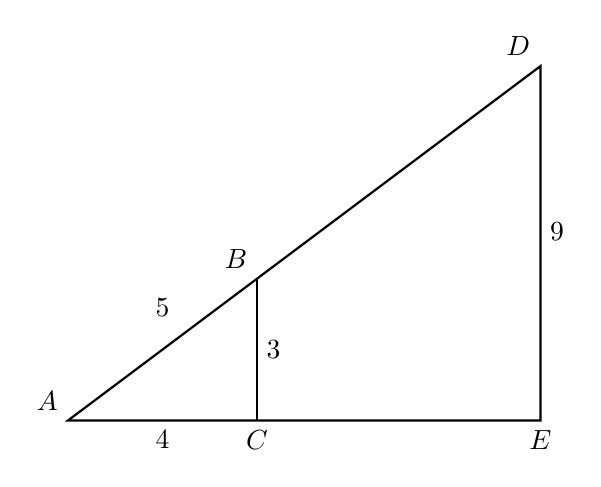
\begin{tikzpicture}[scale=0.6]
        \draw [-, thick] (0,0) node[above left]{$A$}--
        (10,0) node[below]{$E$}--
        (10,7.5) node[above left]{$D$}--cycle;
        \draw [thick] (4,0)--(4,3);
        \node at (4,0) [below]{$C$};
        \node at (4,3) [above left]{$B$};
        \node at (2, 0) [below]{$4$};
        \node at (2, 2) [above]{$5$};
        \node at (10, 4) [right]{$9$};
        \node at (4, 1.5) [right]{$3$};
      \end{tikzpicture}
    \end{flushright} \vspace{0.5cm}

    \item Given $\triangle ABC \sim \triangle DEF$. $m\angle A = 40^\circ$ and $m\angle E = 35^\circ$. Find the measure of $\angle C$. \\*[0.25cm] (\emph{hint: the order of corresponding letters match}) \vspace{2.5cm}

    \item Translate $\triangle ABC$ by $(x,y) \rightarrow (x-4, y+2)$. Make a table of the coordinates and plot and label the image on the axes.
    \begin{flushright}
        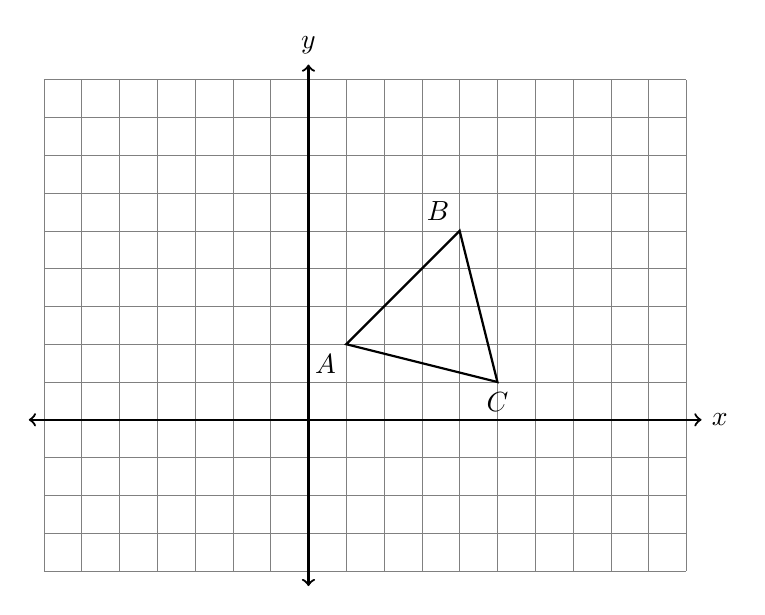
\begin{tikzpicture}[scale=.48]
        \draw [help lines] (-7,-4) grid (10,9);
        \draw [thick, <->] (-7.4,0) -- (10.4,0) node [right] {$x$};
        \draw [thick, <->] (0,-4.4)--(0,9.4) node [above] {$y$};  
        \draw [thick]
          (1,2) node[below left] {$A$}--
          (4,5) node[above left] {$B$}--
          (5,1) node[below] {$C$}--cycle;  
      \end{tikzpicture}
    \end{flushright}
 
\newpage
\item Solve for $y$, then graph and label, marking the intersection as an ordered pair.
        \vspace{0.25cm}
        \begin{multicols}{2}
          $x + 2y =  4$\\
          $\displaystyle \frac{1}{2} x -y = 4$
        \end{multicols}
        \vspace{4cm}

    \begin{center} %4 quadrant regents grid w T-Chart
    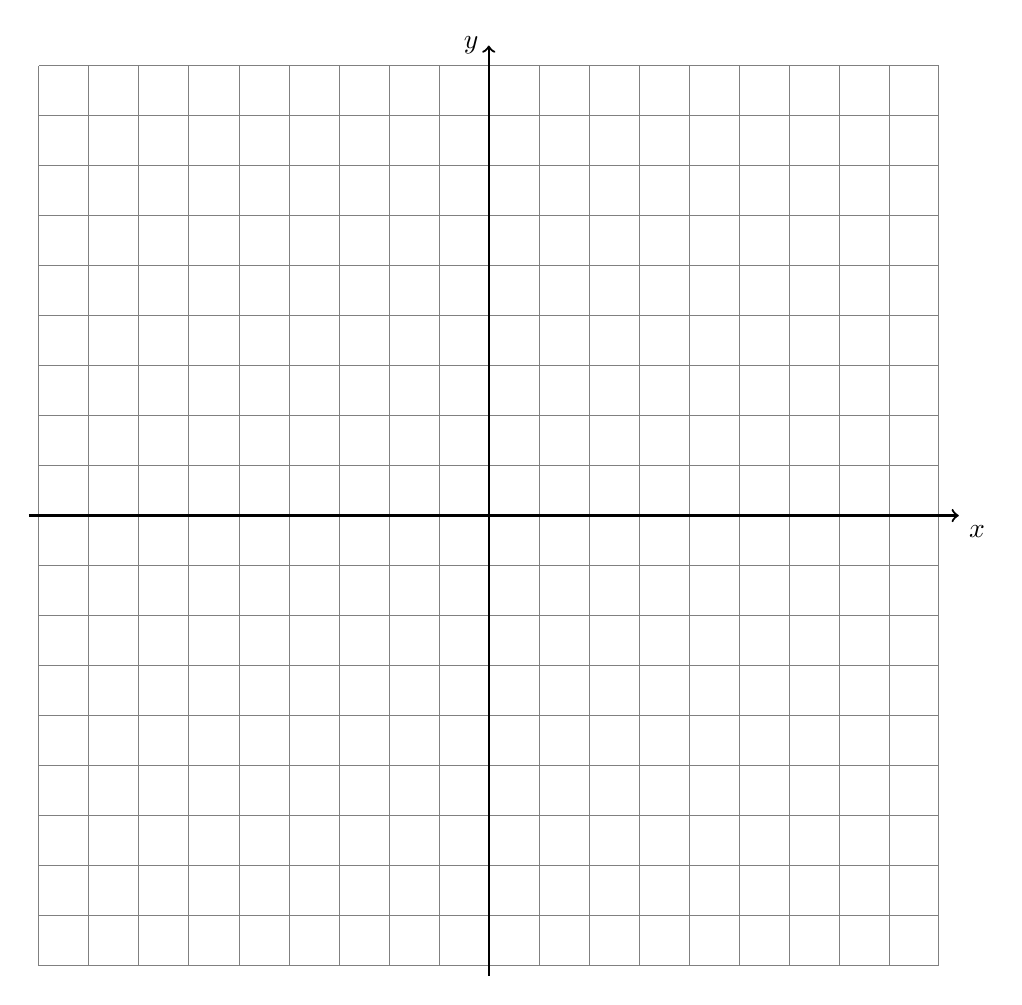
\begin{tikzpicture}[scale=.635]
      \draw [help lines] (-9,-9) grid (9,9);
      \draw [thick, ->] (-9.2,0) -- (9.4,0) node [below right] {$x$};
      \draw [thick, ->] (0,-9.2)--(0,9.4) node [left] {$y$};
    \end{tikzpicture}
    \end{center}

\newpage
  \item Given two parallel lines and a transversal, as shown below.
  \begin{center}
  \begin{tikzpicture}
    \draw [<->, thick] (1,2)--(9,2);
    \draw [<->, thick] (0,0)--(8,0);
    \draw [<->, thick] (4,-1)--(5.5,3);
    \node at (4.5,0.3) [left]{$5$};
    \node at (4.5,0.3) [right]{$6$};
    \node at (4.3,-0.3) [left]{$7$};
    \node at (4.3,-0.3) [right]{$8$};
    \node at (5.2,2) [above left]{$1$};
    \node at (5.2,2) [above right]{$2$};
    \node at (5,2) [below left]{$3$};
    \node at (5,2) [below right]{$4$};
  \end{tikzpicture}
  \end{center}
  \begin{enumerate}
    \item State the angle corresponding with $\angle 1$. \vspace{0.5cm}
    \item What theorem would justify $m\angle 4 + m\angle 6 =180^\circ$? \rule{5cm}{0.15mm} \vspace{0.5cm}
    \item What theorem would justify $\angle 3 \cong \angle 6$? \rule{7cm}{0.15mm} \vspace{0.5cm}
    \item Given $m\angle 1 = 108^\circ$ and $m\angle 8 = (4x-16)^\circ$. Find $x$. \vspace{4.5cm}
  \end{enumerate}

  \item The side $\overline{AB}$ of triangle $ABC$ is extended and an altitude to the vertex $C$ is drawn, as shown below. The triangle's height is $h=7.2$ and its base measures $AB=12.4$. Find the area of the triangle.
    \begin{flushright}
      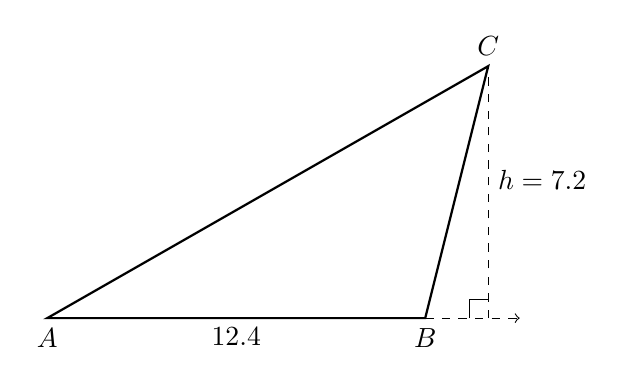
\begin{tikzpicture}[scale=0.8]
        \draw [thick]
          (0,0)node[below]{$A$}--
          (6,0)node[below]{$B$}--
          (7,4)node[above]{$C$} --cycle;
      \draw [dashed] (7,0)--(7,4);
      \draw [dashed, ->] (6,0)--(7.5,0);
      \draw (7,0)++(-0.3,0)--++(0,0.3)--+(0.3,0);
      \node at (7,2.2)[right]{$h=7.2$};
      \node at (3,0)[below]{$12.4$};
      \end{tikzpicture}
    \end{flushright}

\newpage
\subsubsection*{Do Not Solve! Make a drawing on the right, an equation to the left, and circle where it states what to find.}
\vspace{0.5cm}

  \item The point $Q$ is the midpoint of $\overline{PR}$, $PQ=11$, and $QR=2x+1$. Find ${x}$.
  \vspace{4cm}
  
  \item Given $\overline{PQR}$, with $PQ=3x-7$, $QR=x+3$, and $PR=12$. Find ${x}$.
  \vspace{4cm}
  
  \item Given that $Q$ bisects $\overline{PR}$. $PQ=2x-5$, $PR=42$. Find ${x}$.
  \vspace{4cm}

  \item The points $P$, $Q$, and $R$ are collinear, with $PQ=x+4$ and $PR=27$. $\overline{QR}$ is twice the length of $\overline{PQ}$. Find ${x}$.

\newpage
    \item Given isosceles $\triangle TUV$ with $\overline{TU} \cong \overline{UV}$ and $m\angle U = 50$. Mark the triangle in the diagram and find $m\angle U$ and $m\angle V$.
  \begin{flushright}
    (\emph{the diagram is not to scale})\\
  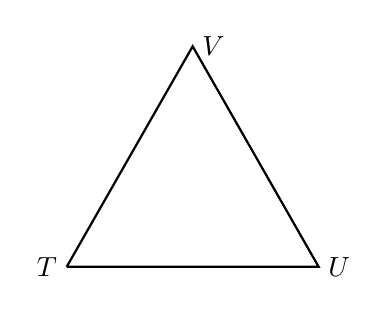
\begin{tikzpicture}[scale=0.8]
    \draw [thick](0,0)--(4,0)--(2,3.5)--(0,0);
    \node at (0,0) [left]{$T$};
    \node at (4,0) [right]{$U$};
    \node at (2,3.5) [right]{$V$};
  \end{tikzpicture}
  \end{flushright}

  \item The points $R$, $S$, and $T$ are collinear, with $RS=4x-8$, $ST=21$, and $RT=6x-1$. \\*[0.25cm]
  Mark the diagram and find ${RT}$. \vspace{0.5cm}
  \begin{flushright}
    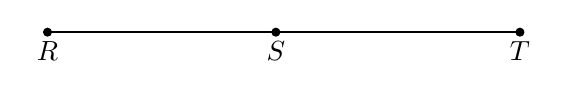
\begin{tikzpicture}
      \draw [-, thick] (0,0)--(6,0);
      \draw [fill] (0,0) circle [radius=0.05] node[below]{$R$};
      \draw [fill] (2.9,0) circle [radius=0.05] node[below]{$S$};
      \draw [fill] (6,0) circle [radius=0.05] node[below]{$T$};
    \end{tikzpicture}
    \end{flushright} \vspace{4cm}

  \item A translation maps $X(2,-7) \rightarrow X'(3,5)$. 
    \begin{enumerate}
      \item What translation was applied (be specific)?  \vspace{2cm}
      \item What is the image of $Y(1,3)$ under the same translation?
      \end{enumerate} \vspace{2cm}
  
\newpage
  \item Given $\triangle ABC$ point $D$ on $\overline{AB}$ and point $E$ on $\overline{BC}$ such that $\triangle ABC \sim \triangle DBE$. \\*[0.25cm]
  Given $AB=15$, $BC=10$, and $AD=9$. Mark the lengths on the triangle, showing $DB$ as well. \\*[0.25cm] Find the length of $\overline{BE}$.
    \begin{flushright}
      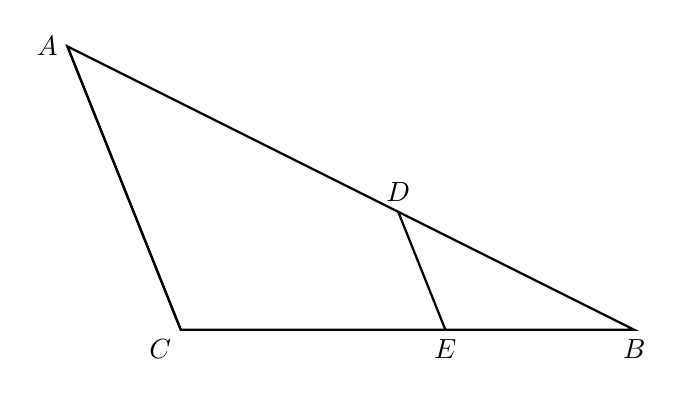
\begin{tikzpicture}[scale=0.6]
        \coordinate [label=left:$A$](A) at (-12,6);
        \coordinate [label=below:$B$](B) at (0, 0);
        \coordinate [label=below left:$C$](C) at (-9.6,0);
        \coordinate [label=above:$D$](D) at (-5, 2.5);
        \coordinate [label=below:$E$](E) at (-4,0);
        \draw [thick] (A)--(B)--(C)--cycle;
        \draw [thick] (A)--(C);
        \draw [thick] (D)--(E);
      \end{tikzpicture}
    \end{flushright} \vspace{3cm}

  \item $\triangle ABC$ is shown with vertices $A(2,-3)$, $B(-2,3)$, and $C(3,4)$. Translate the triangle to the left three units and up two units. Write down its coordinates in a table and plot and label it on the graph.
    \begin{flushright}
      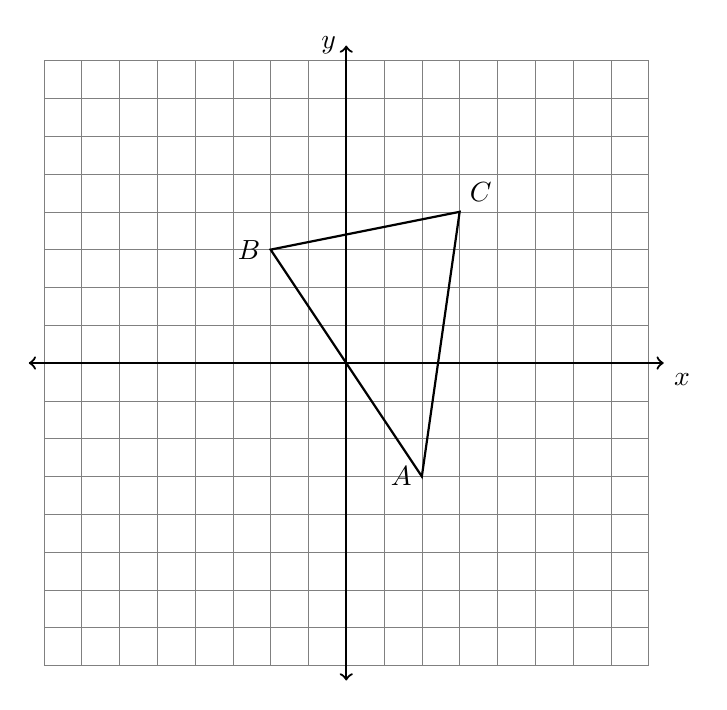
\begin{tikzpicture}[scale=.48]
        \draw [help lines] (-8,-8) grid (8,8);
        \draw [thick, <->] (-8.4,0) -- (8.4,0) node [below right] {$x$};
        \draw [thick, <->] (0,-8.4)--(0,8.4) node [left] {$y$};
        \draw [thick] (2,-3) node[left] {$A$}--
          (-2,3) node[left] {$B$}--
          (3,4) node[above right] {$C$}--
          cycle;
      \end{tikzpicture}
      \end{flushright}

\newpage
  \item The shape shown below is composed of straight lines and right angles, with some lengths as marked. Find the area of the figure. (the figure is not drawn to scale)
  \begin{flushleft}
  \begin{tikzpicture}[scale=0.5]
  \draw [-, thick] (0,0)--(13,0)--(13,3)--(9,3)--(9,9)--
  (0,9)--(0,7)--(4,7)--(4,3)--(0,3)--cycle;
  %\draw [fill] (0,0) circle [radius=0.05] node[left]{$A$};
  %\draw [fill] (7,0) circle [radius=0.05] node[right]{$B$};
  %\draw [fill] (7,2) circle [radius=0.05] node[right]{$C$};
  %\draw [fill] (0,2) circle [radius=0.05] node[left]{$D$};
  \node at (4.5, 5){4};
  \node at (2, 2.5){4};
  \node at (8.5, 6){6};
  \node at (11, 2.5){4};
  \node at (6.5, -0.5){13};
  \node at (13.5, 1.5){3};
  %\node at (13.5, 8){2};
  \end{tikzpicture}
  \end{flushleft} \vspace{3cm}

  \item Given isosceles $\triangle RSU$ with $\overline{US} \cong \overline{RS}$. If $m\angle UST=150$ find $m\angle U$.
  \begin{flushright}
  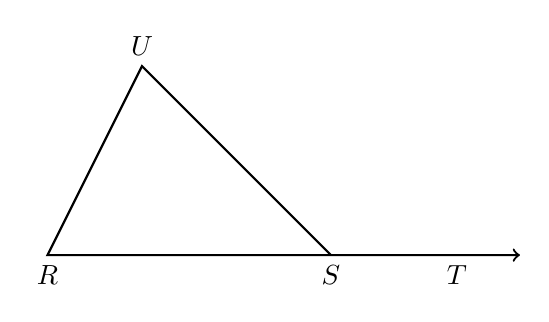
\begin{tikzpicture}[scale=0.8]
    %\draw [->, thick] (0,0)--(5,5);
    \draw [<-, thick] (8,0)--
      (7,0) node[below]{$T$}--
      (0.5,0) node[below]{$R$}--
      (2,3) node[above]{$U$}--
      (5,0) node[below]{$S$};
  \end{tikzpicture}
  \end{flushright} \vspace{1cm}

\newpage
  \item One side of the $\triangle ABC$ has a length $AB=15$. The triangle's area is $71 \frac{1}{4}$. Find the length of the altitude $h$ of the triangle.\\[0.5cm]
  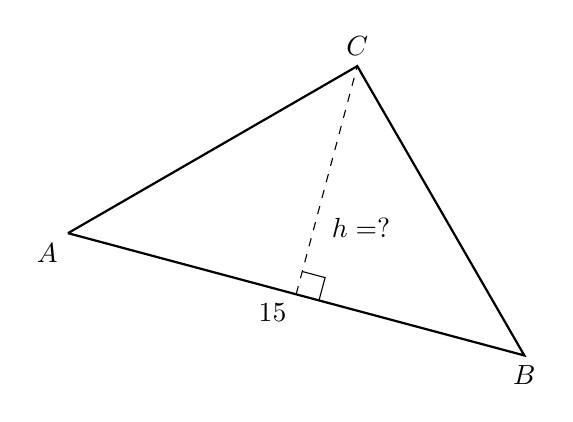
\begin{tikzpicture}[scale=1, rotate=-15]
  \draw [thick]
  (2,0)node[below left]{$A$}--
  (8,0)node[below]{$B$}--
  (5,3)node[above]{$C$} --(2,0);
  \draw [dashed] (5,0)--(5,3);
  \draw (5,0)++(0.3,0)--++(0,0.3)--+(-0.3,0);
  \node at (5.1,0.9)[right]{$h=?$};
  \node at (5,0)[below left]{$15$};
  \end{tikzpicture} \vspace{3.0cm}

  \item The point $K$ is the midpoint of $\overline{JL}$, $JK=3x+11$, and $JL=9x+1$. Mark the line on the right and find ${JK}$.  \vspace{1cm}
  \begin{flushright}
    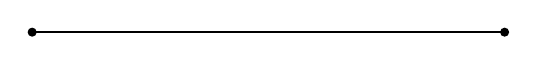
\begin{tikzpicture}
      \draw [-, thick] (0,0)--(6,0);
      \draw [fill] (0,0) circle [radius=0.05];
      \draw [fill] (6,0) circle [radius=0.05];
    \end{tikzpicture}
    \end{flushright} \vspace{2cm}

\end{enumerate}
\end{document}
